\documentclass[border=10pt]{standalone}
\usepackage{pgfplots}
\pgfplotsset{compat=1.18}
\begin{document}
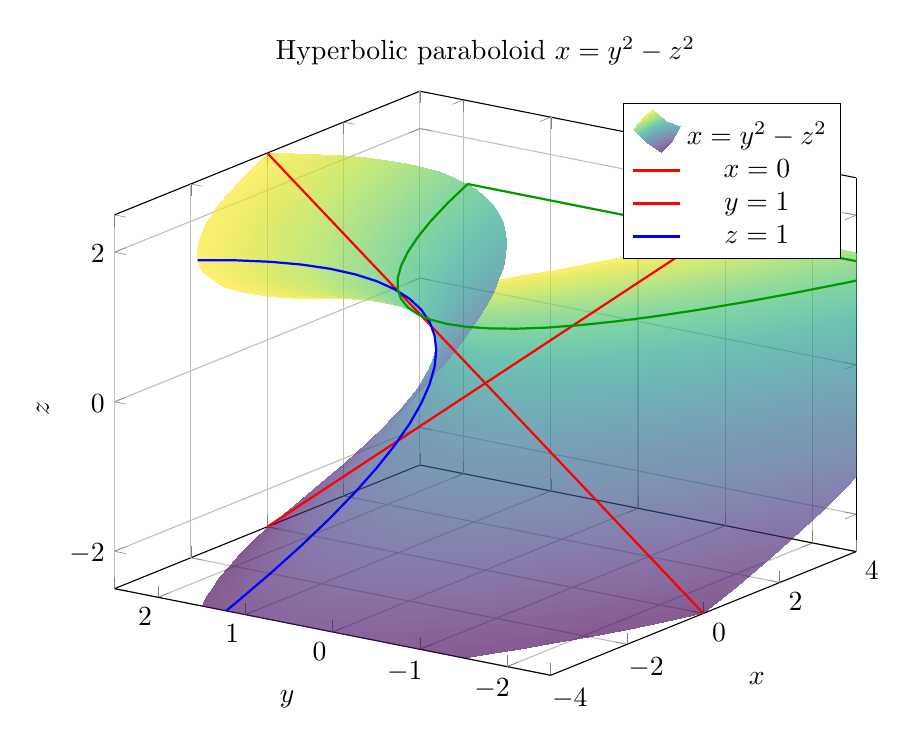
\begin{tikzpicture}
\begin{axis}[
    width=11cm, height=9cm,
    view={-55}{22},
    xlabel=$x$, ylabel=$y$, zlabel=$z$,
    title={Hyperbolic paraboloid $x=y^2-z^2$},
    grid=major,
    colormap/viridis,
    xmin=-4, xmax=4,
    ymin=-2.5, ymax=2.5,
    zmin=-2.5, zmax=2.5
]
\addplot3[
    surf,
    domain=-2.5:2.5,
    y domain=-2.5:2.5,
    samples=35,
    shader=interp,
    opacity=0.65
] ({x*x-y*y},{x},{y});

\addplot3[domain=-2.5:2.5, red, thick] ({0},{x},{x});
\addplot3[domain=-2.5:2.5, red, thick] ({0},{x},{-x});
\addplot3[domain=-2.5:2.5, blue, thick] ({1-y*y},{1},{y});
\addplot3[domain=-2.5:2.5, green!60!black, thick] ({x*x-1},{x},{1});

\legend{$x=y^2-z^2$,$x=0$,$y=1$,$z=1$}
\end{axis}
\end{tikzpicture}
\end{document}